%%%%%%%%%%%%%%%%%%%%%%%%%%%%%%%%%%%%%%%%%
% Structured General Purpose Assignment
% LaTeX Template
%
% This template has been downloaded from:
% http://www.latextemplates.com
%
% Original author:
% Ted Pavlic (http://www.tedpavlic.com)
%
% Note:
% The \lipsum[#] commands throughout this template generate dummy text
% to fill the template out. These commands should all be removed when 
% writing assignment content.
%
%%%%%%%%%%%%%%%%%%%%%%%%%%%%%%%%%%%%%%%%%

\documentclass{article}

\usepackage{fancyhdr} % Required for custom headers
\usepackage{lastpage} % Required to determine the last page for the footer
\usepackage{extramarks} % Required for headers and footers
\usepackage{graphicx} % Required to insert images
\usepackage[utf8]{inputenc}

% Margins
\topmargin=-0.45in
\evensidemargin=0in
\oddsidemargin=0in
\textwidth=6.5in
\textheight=9.0in
\headsep=0.25in 

\linespread{1.1} % Line spacing



\setlength\parindent{0pt} % Removes all indentation from paragraphs

%----------------------------------------------------------------------------------------
%	DOCUMENT STRUCTURE COMMANDS
%	Skip this unless you know what you're doing
%----------------------------------------------------------------------------------------

% Header and footer for when a page split occurs within a problem environment
\newcommand{\enterProblemHeader}[1]{
\nobreak\extramarks{#1}{#1 continued on next page\ldots}\nobreak
\nobreak\extramarks{#1 (continued)}{#1 continued on next page\ldots}\nobreak
}

% Header and footer for when a page split occurs between problem environments
\newcommand{\exitProblemHeader}[1]{
\nobreak\extramarks{#1 (continued)}{#1 continued on next page\ldots}\nobreak
\nobreak\extramarks{#1}{}\nobreak
}

\setcounter{secnumdepth}{0} % Removes default section numbers
\newcounter{homeworkProblemCounter} % Creates a counter to keep track of the number of problems

%----------------------------------------------------------------------------------------
%	NAME AND CLASS SECTION
%----------------------------------------------------------------------------------------

\newcommand{\lessonNumber}[1]{Lezione\ \##1} % Assignment title
\newcommand{\lessonDate}[4]{#1,\ #2\ #3\ #4} % Due date
\newcommand{\lessonCourse}[1]{#1} % Course/class
\newcommand{\lessonTime}[1]{#1} % Class/lecture time
\newcommand{\lessonTeacher}[1]{#1} % Teacher/lecturer
\newcommand{\lessonAuthor}[1]{#1} % Your name
\begin{document}
\section{Qualità del software(6)}

L'attività di \textbf{analisi dei requisiti} è importantissima, comporta molte competenze ed è complessa, per cui viene chiamata \textbf{Ingegneria dei requisiti}. Un requisito può essere visto da due lati:

\begin{itemize}

	\item \textbf{Vista cliente:} qual'è il bisogno da soddisfare;
	\item \textbf{Vista fornitore:} come deve essere la soluzione del bisogno.

\end{itemize}

Dovrò prima interrogare gli stakeholders e poi chiedermi cosa serve a me per soddisfare quei requisiti. Quando queste due cose sono soddisfatte avrò soddisfatto il \textbf{requisito utente}. Sui requisiti si effettua \textit{breakdown}, spezzamento, perchè rende più facile verificare che siano soddisfatti.\\

Dei processi di supporto al ciclo di vita sono:
\begin{itemize}

	\item La \textbf{Verifica:} faccio in modo che tutte le attività assegnate introducano la più piccola possibilità di errore, rivolta principalmente ai processi (modo di lavorare);
	\item la \textbf{Validazione:} accertare che il prodotto realizzato corrisponda alle attese.

\end{itemize}

Questi due processi formano la \textbf{qualifica}.

Si lavora sempre secondo regole di procedura. Devono esistere delle regole prima di iniziare il lavoro. Avremo alla fine specializzato un prodotto che soddisfa i requisiti iniziali e le sue aspettative. Un lavoro \textbf{verificato} è un lavoro fatto nel modo giusto e secondo le regole date. \\
Molti dei sistemi al giorno d'oggi sono detti \textbf{socio-tecnici}, hanno come dato rilevante l'elemento \textbf{umano}, che è come la persona userà quel prodotto. Chiedersi che ruolo ha l'utente umano nel sistema è parte fondamentale dell'AR. In ogni sistema organizzato c'è uno \textit{sportello} rivolto all'umano; molto spesso si chiama \textit{front office} (interfaccia utente). L'opposizione è il \textit{back office} in cui si prepara ciò che andrà al front office (es. database). Devo capire entrambe queste parti per realizzare un sistema socio-tecnico. E' molto raro progettare un sistema esclusivamente tecnico. Ci sono due fasi:

\begin{itemize}

	\item \textbf{Analisi:} analisi dei bisogni e delle fonti, classificazione dei requisiti, visione UC, confronto con le fonti(committente, sottofornitori);
	\item \textbf{Validazione:} successiva all'Analisi, predispone la revisione interna/esterna, di prove e dimostrazioni.

\end{itemize}

In questa fase i processi coinvolti sono la \textbf{Documentazione} e la \textbf{Gestione e manutenzione dei prodotti}. Questo tipo di analisi dei requisiti da luogo a un ciclo di vita simile:\\
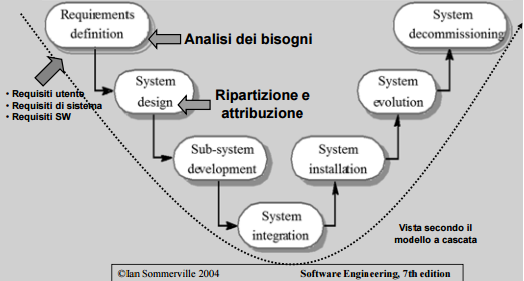
\includegraphics[width=0.75\columnwidth]{img1}
\\
Questo rappresentato è un modello sequenziale con le base line, condizione di massima sicurezza. In opposto con un modello \textit{Agile} non fissiamo la base line ma abbiamo i requisiti dal confronto con il cliente.

I prodotti attesi alla fine di questa fase sono molteplici:

\begin{itemize}
	\item Dall'analisi dei bisogni e delle fonti:
	\begin{itemize}
		\item Capitolato d'appalto (unico di responsabilità del cliente, definisce i requisiti)
		\item Studio di fattibilità
		\item Analisi dei requisiti
	\end{itemize}
	\item Dalla ripartizione dei requisiti
	\begin{itemize}
		\item Specifica tecnica (modellazione architetturale del SW con caratterizzazione architetturale dei componenti)
	\end{itemize}
\end{itemize}

Per produrli si può  ricorrere a due tipi di approccio:
\begin{itemize}
	\item \textbf{Approccio Funzionale}
	\item \textbf{Approccio Object-Oriented}
\end{itemize}
%slide 17 ingegneria dei requisiti
\end{document}